\begin{figure}
    \centering
    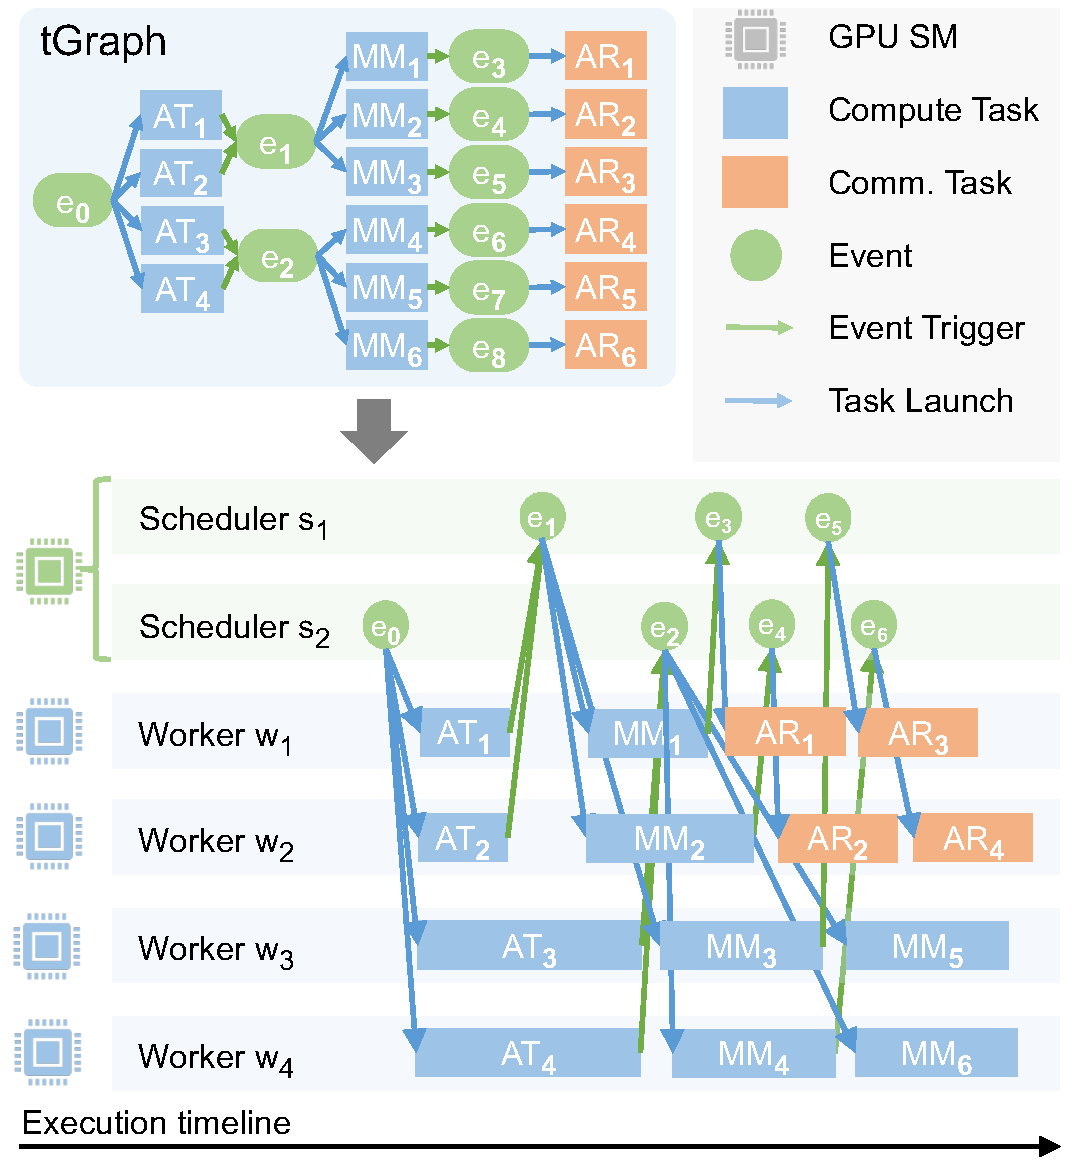
\includegraphics[scale=0.4]{figs/execution_graph.pdf}
    \vspace{\captionvspace}
    \caption{\Sys 的事件驱动执行模型。圆形表示事件，蓝色（或橙色）矩形分别表示计算任务（或通信任务）。从事件指向任务的边表示任务发射，从任务指向事件的边表示该任务会触发对应事件。图中的 {\tt AT}、{\tt MM} 与 {\tt AR} 分别表示 attention、matrix multiplication 与 AllReduce。}
    \vspace{\captionvspace}
    \label{fig:execution}
\end{figure}

\section{核内并行运行时}
\label{sec:runtime}

\Sys 采用 {\em 核内并行运行时}，在单个 mega-kernel 内跨全部 SM 执行 \graph。这样的设计既消除了 kernel 发射开销，也使系统能够细粒度控制调度、同步与执行顺序。mega-kernel 一旦启动，就会持续管理计算与通信，直到一次推理工作负载结束。

为了支撑这一执行模式，\sys 会把 GPU 的 SM 划分为 {\em worker} 和 {\em scheduler}。每个 worker 运行在一个物理 SM 上，并维护独立的 {\em task queue}。worker 会不断从队列中取出任务，执行相应的计算或通信，并在任务完成后通知其触发事件。这样的设计既保证了 worker 的高利用率，也支持跨算子的异步执行。

scheduler 以 {\em warp} 为粒度组织，每个 SM 上驻留 4 个 scheduler warp。每个 scheduler 维护一个事件队列，并持续轮询是否有新激活的事件；一旦发现，就把对应任务分发给 worker。worker 与 scheduler 的数量在 kernel 发射时就固定下来，并与 GPU 的物理 SM 数量匹配，从而避免在 kernel 内部进行动态角色切换。

本节余下部分将详细介绍这一核内运行时架构。 \Cref{subsec:event_driven_execution} 描述 \sys 的事件驱动执行模型；\Cref{subsec:task_launch} 比较两种互补的任务发射机制并说明 \sys 如何组合它们；\Cref{subsec:runtime_optimizations} 则介绍若干进一步降低运行时开销的系统优化。

\subsection{事件驱动执行}
\label{subsec:event_driven_execution}

\Sys 使用 {\em 事件驱动} 模型执行 \graph。每个 \graph 都有一个没有任何前置条件的起始事件，例如 \Cref{fig:execution} 中的 $e_0$。该事件最初会被放入某个 scheduler 的事件队列。当 scheduler 取出该事件后，它会发射所有依赖该事件的任务，例如 $AT_1,\ldots,AT_4$。这些任务被分发给 worker 执行，任务结束后，worker 再去通知与之关联的触发事件。

当一个事件的所有前置条件都已完成，并且它收到足够次数的触发后，该事件就会被 {\em 激活}。一旦激活，它就会再次进入某个 scheduler 的事件队列，驱动运行时继续沿着 \graph 向前推进。换言之，在 \sys 中，事件是驱动任务执行的核心机制，这使得系统可以在细粒度上实现完全异步的执行。

\begin{figure}
    \centering
    \subfloat[即时（JIT）任务发射。]{
    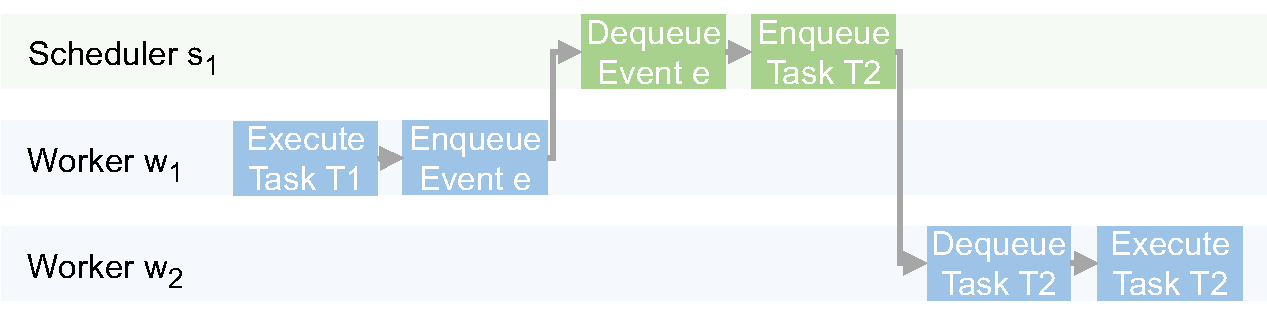
\includegraphics[scale=0.38]{figs/jit_launch.pdf}
    \label{fig:jit_launch}
    }
    \\
    \subfloat[提前（AOT）任务发射。]{
    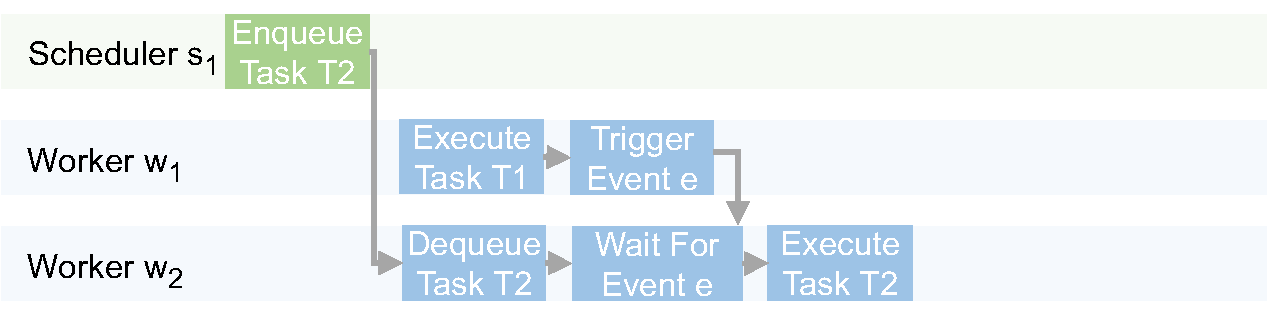
\includegraphics[scale=0.38]{figs/aot_launch.pdf}
    \label{fig:aot_launch}
    }
    \vspace{\captionvspace}
    \caption{JIT 与 AOT 两种任务发射方式的比较。}
    \vspace{\captionvspace}
    \label{fig:aot_and_jit}
\end{figure}

\subsection{混合任务发射}
\label{subsec:task_launch}

一个任务可以通过两种方式被放入 worker 的任务队列：{\em just-in-time}（JIT）或 {\em ahead-of-time}（AOT）。在 JIT 模式下，scheduler 只有在任务的依赖事件完全激活后，才会把该任务分配给某个 worker，因此任务一旦入队就可以立刻执行。相反，在 AOT 模式下，运行时会在前驱事件尚未激活之前，就把任务预先放入 worker 的本地队列；worker 会在本地等待依赖满足后再执行。

这两种方式各有优势。JIT 更利于应对负载不均衡，因为 scheduler 能在依赖满足的瞬间根据当前系统状态选择空闲 worker。例如现代 LLM 中的 attention 算子往往具有明显的数据相关执行时间波动，JIT 能更好地适配这种不均匀性。AOT 的优势则在于它减少了任务真正可运行时的调度路径长度：任务已经在 worker 本地排好队，只要依赖满足就能立即开始，因而有助于降低延迟并减少 scheduler 压力。

\Sys 的做法是结合二者，使用 {\em 混合任务发射}。对于那些执行时间稳定、负载容易预测、并且位于关键路径上的任务，\sys 更倾向于使用 AOT，从而减少等待 scheduler 再次介入的开销；对于执行时间波动较大、或需要动态负载均衡的任务，则更适合使用 JIT，以便系统根据运行时状态灵活分配。通过这种组合，\sys 同时获得了 AOT 的低延迟和 JIT 的弹性调度能力。

\subsection{运行时优化}
\label{subsec:runtime_optimizations}
本小节介绍一组用于最小化 \sys 运行时开销的优化。

\paragraph{分页共享内存抽象。}
在传统 CUDA 或 Triton 编程模型中，shared memory 是 thread block 私有的高速片上存储，并且只在 kernel 生命周期内存在。因此，当前按算子逐核执行的模型通常默认每个 kernel 可以 {\em 独占} 整块 shared memory。

但这种独占式设计会阻碍跨任务软件流水，因为后一任务的数据加载阶段往往需要与前一任务的计算阶段重叠，而两者都需要访问 shared memory。为了解决这个问题，\Sys 引入了 {\em 分页共享内存} 抽象。系统把 shared memory 划分为多个固定大小的页，任务实现则被改写为在这些页面上操作，而不再假设自己独占一整块单体共享内存。任务可以按需 {\em 获取} 一个或多个页，在不再需要时 {\em 释放} 它们；一旦开始释放页面，就不能再申请新的页面，以保证使用模式单调、便于调度。当当前任务释放页面后，\sys 就能立即把这些可用页面预分配给下一个任务，并启动数据预取。

\paragraph{跨任务软件流水。}
为了让同一 worker 上连续执行的任务之间也能形成软件流水（\Cref{subsec:gpu-programming-model}），\sys 将每个任务拆成 {\em 预加载} 和 {\em 计算} 两个阶段。预加载阶段负责把输入张量的一部分从 device memory 拉入 shared memory，并启动任务内部的软件流水，但本身不进行计算。

当满足两个条件时，\Sys 会机会式地把当前任务 $T_1$ 的计算阶段与后继任务 $T_2$ 的预加载阶段重叠起来：(1) $T_1$ 已经发出了自己所需的全部数据传输指令；(2) 当前存在足够的 shared-memory 页面供 $T_2$ 预加载使用。这样的流水不会破坏 $T_1$ 的执行正确性，因为 \sys 会插入适当的 SM 内同步屏障，确保 $T_2$ 的内存传输不会与 $T_1$ 尚未完成的数据搬运冲突。

\paragraph{任务描述预取。}
每个 worker 都在 device memory 中维护 JIT 和 AOT 两类任务队列。每个任务还对应一个描述符，用于记录输入张量、输出张量及其配置参数；在当前实现中，一个任务描述占 352 字节（见 \Cref{sec:impl}）。为了降低任务入队与出队延迟，并隐藏读取 device memory 的成本，\sys 使用一个轻量级预取机制，在真正需要之前就把后续任务的描述符拉入 shared memory。
